\documentclass[11pt,a4paper]{book}
\usepackage[brazilian]{babel}
\usepackage[utf8]{inputenc}
\usepackage[T1]{fontenc}
\usepackage[inline]{enumitem}
\usepackage{xcolor}
\usepackage{listings}
\usepackage{graphicx}
\usepackage{multicol}
\usepackage{amsmath}
\usepackage{amssymb}

\definecolor{mGreen}{rgb}{0,0.6,0}
\definecolor{mGray}{rgb}{0.5,0.5,0.5}
\definecolor{mPurple}{rgb}{0.58,0,0.82}
\definecolor{backgroundColour}{rgb}{0.95,0.95,0.92}

\lstdefinestyle{CStyle}{
    backgroundcolor=\color{backgroundColour},   
    commentstyle=\color{mGreen},
    keywordstyle=\textbf{\color{black}},
    numberstyle=\tiny\color{mGray},
    stringstyle=\color{mPurple},
    basicstyle=\footnotesize,
    breakatwhitespace=false,         
    breaklines=true,                 
    captionpos=b,                    
    keepspaces=true,                 
    numbers=left,                    
    numbersep=5pt,                  
    showspaces=false,                
    showstringspaces=false,
    showtabs=false,                  
    tabsize=2,
    frame=single,
    escapeinside={(*}{*)},
    language=C
}

\makeatletter
% This command ignores the optional argument for itemize and enumerate lists
\newcommand{\inlineitem}[1][]{%
\ifnum\enit@type=\tw@
    {\descriptionlabel{#1}}
  \hspace{\labelsep}
\else
  \ifnum\enit@type=\z@
       \refstepcounter{\@listctr}\fi
    \quad\@itemlabel\hspace{\labelsep}
\fi}
\makeatother

\newcommand{\onestaritem}{\refstepcounter{enumi}\item[$*$\theenumi.]}
\newcommand{\twostaritem}{\refstepcounter{enumi}\item[$**$\theenumi.]}

\title{Lista 7: Fundamentos Estatísticos para Ciência dos Dados}
\author{Ricardo Pagoto Marinho}

\begin{document}
\maketitle
	\begin{enumerate}
		\item Exercício 1.6:
		\begin{enumerate}[label=\alph*)]
			\item Coloquei a tabela em um arquivo ".csv".
			\begin{lstlisting}	
tab<-read.csv("tab1.csv",sep=";")
par(mfrow=c(2,4))
dotchart(tab$Wind,xlab = "Wind")
dotchart(tab$radiation,xlab="radiation")
dotchart(tab$CO,xlab="CO")
dotchart(tab$NO,xlab="NO")
dotchart(tab$NO2,xlab="NO2")
dotchart(tab$O3,xlab="O3")
dotchart(tab$HC,xlab="HC")
			\end{lstlisting}
		
			A Figura~\ref{fig:fig1} mostra os diagramas marginais das variáveis coletadas.
		
			\begin{figure}[h]
				\centering
				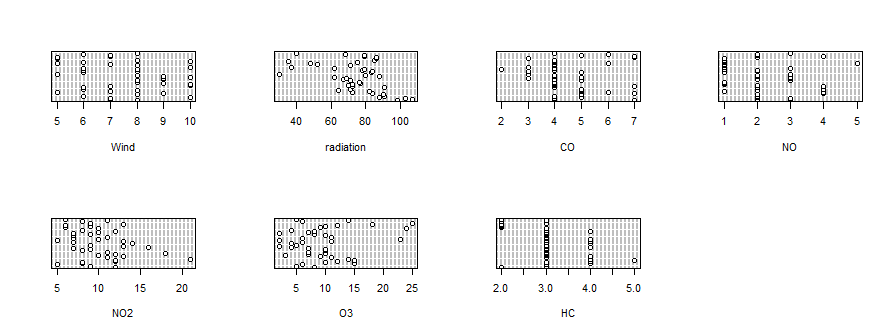
\includegraphics[height=10cm, width=0.99\textwidth]{Rplot.png}
				\caption{Diagramas marginais das 7 variáveis}
				\label{fig:fig1}
			\end{figure}
			
			\item $\bar{x}$:
			\begin{lstlisting}
m<-apply(tab,2,mean)
m
     Wind radiation        CO        NO       NO2 
 7.500000 73.857143  4.547619  2.190476 10.047619 
       O3        HC 
 9.404762  3.095238 
			\end{lstlisting}
			
			Ou seja:
			
			\begin{eqnarray*}
				\bar{x}=\left[
				\begin{tabular}{c}
					7.500000\\
					73.857143\\
					4.547619\\
					2.190476\\
					10.047619\\
					9.404762\\
					3.095238
				\end{tabular}
				\right]
			\end{eqnarray*}
			
			Para calcular a matriz de covariância $S_7$, o seguinte cálculo foi feito:
			\begin{lstlisting}
s<-matrix(0,7,7)
for(i in 1:7){
    for(j in 1:7){
        s[i,j]=sum((tab[,i]-x[i])*(tab[,j]-x[j]))/42
    }
}
			\end{lstlisting}
			
			Assim a matriz é a seguinte:
			
			\begin{eqnarray*}
				S_n=\left[
				\resizebox{\textwidth}{!}{%
				\begin{tabular}{c c c c c c c}
					32.6904762 & 387 & 2.6428571 & 0.5952381 & 21.690476 & 11.0476190 & -10.3095238\\
					387 & 5314.09524 & 42.6190476 & 12.1428571 & 293.404762 & 200.4523810 & -134.3571429\\
					 2.6428571 & 42.61905 & 1.7857143 & 0.7619048 & 4.476190 & 4.0714286 & -0.9047619 \\
					 0.5952381 & 12.14286 & 0.7619048 & 1.1904762 & 1.833333 & -0.3333333 & -0.1904762\\
					 21.6904762 & 293.40476 & 4.4761905 & 1.8333333 & 27.476190 & 12.7857143 &  -6.6904762\\
					11.0476190 & 200.45238&  4.0714286& -0.3333333&  12.785714 & 36.0238095 &  -4.0000000\\
					-10.3095238& -134.35714& -0.9047619& -0.1904762 & -6.690476&  -4.0000000  &  4.0952381
				\end{tabular}}
				\right]
			\end{eqnarray*}
			
			Como é possível observar, a matriz é simétrica, ou seja, $s_{ij}=s_{ji}$.
			
			Por fim, a matriz de correlação \textbf{R} foi calculada da seguinte forma:
			
			\begin{lstlisting}
r<-matrix(0,7,7)
for(i in 1:7){
    for(j in 1:7){
        r[i,j]=s[i,j]/(sqrt(s[i,i])*sqrt(s[j,j]))
    }
}
			\end{lstlisting}
			
			A matriz \textbf{R} ficou da seguinte forma:
			\begin{eqnarray*}
				R=\left[
				\resizebox{\textwidth}{!}{%
				\begin{tabular}{c c c c c c c}
					1.00000000 & 0.9285081 & 0.3459052 & 0.09541568 & 0.7237360&  0.32193133& -0.89102195\\
					0.92850805 & 1.0000000 & 0.4375051 & 0.15266724&  0.7678462 & 0.45814372& -0.91076538\\
					0.34590519 & 0.4375051 & 1.0000000 & 0.52255781 & 0.6390345 & 0.50762852& -0.33457134\\
					0.09541568 & 0.1526672 & 0.5225578 & 1.00000000 & 0.3205552& -0.05090068& -0.08626622\\
					0.72373605 &0.7678462 & 0.6390345 & 0.32055519 & 1.0000000 & 0.40639833 &-0.63072376\\
					0.32193133 & 0.4581437 & 0.5076285& -0.05090068 & 0.4063983&  1.00000000& -0.32932568\\
					-0.89102195 & -0.9107654& -0.3345713& -0.08626622& -0.6307238& -0.32932568 & 1.00000000
				\end{tabular}}
				\right]
			\end{eqnarray*}
			
			A matriz de correlação é caracterizada pela diagonal principal igual a 1, simétrica e todos os valores entre [-1,1], como é possível observar.
			
			Para calcular $d^2(y,\mu)$, a seguinte função foi criada:
			
			\begin{lstlisting}
est_dist = function(table){
    cov_matrix=cov(table)
    mu=apply(table,2,mean)
    return(mahalanobis(table,center = mu,cov = cov_matrix))
}
			\end{lstlisting}
			
			A Figura~\ref{fig:fig2} mostra o histograma criado com a função e sua distribuição de probabilidade.			
			
			\begin{figure}[h]
			\centering
			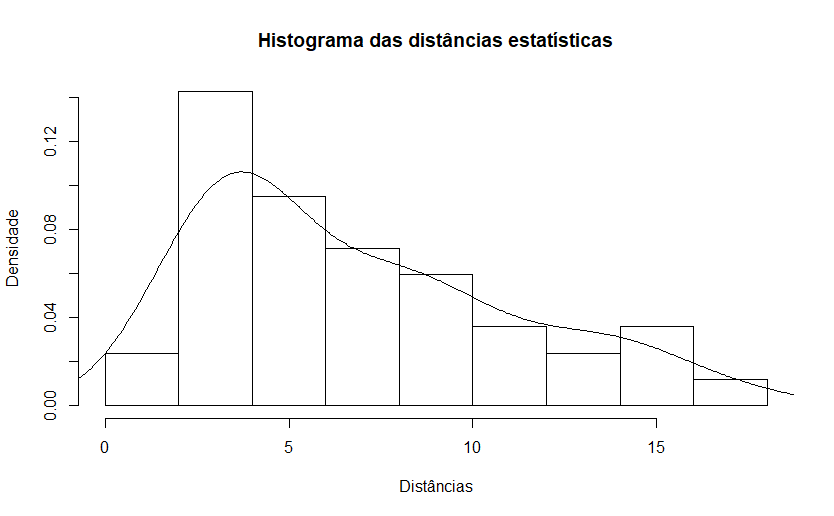
\includegraphics[height=7cm]{hist.png}
			\caption{Histograma}
			\label{fig:fig2}
			\end{figure}
			
			O seguinte código foi utilizado para verificar, através do teste qui-quadrado, se a distribuição utilizada foi adequada:
			
			\begin{lstlisting}
sum(d2<=qchisq(0.95,7))/42
0.9285714
			\end{lstlisting}
			
			Como a porcentagem de valores que são menores que o teste é próxima a 95\%, podemos afirmar que a distribuição é adequada.
		\end{enumerate}
		\item
		\begin{enumerate}[label=\alph*)]
			\item
			\begin{lstlisting}
A=matrix(c(9,-2,-2,6),2,2)
eigen(A,symmetric = FALSE)
eigen() decomposition
$values
[1] 10  5
$vectors
           [,1]      [,2]
[1,]  0.8944272 0.4472136
[2,] -0.4472136 0.8944272
			\end{lstlisting}
			\item A decomposição espectral de A se dá da seguinte maneira:
			
			\begin{eqnarray*}
				A=X\Lambda X^{-1}
			\end{eqnarray*}
			
			Onde X é a matriz de autovetores de A e $\Lambda$ é uma matriz diagonal com os autovalores de A.
			Então:
			\begin{eqnarray*}
				A=&\left[
				\begin{tabular}{c c}
				9&-2\\
				-2&6
				\end{tabular}
				\right]\\
				X=&\left[
				\begin{tabular}{c c}
				 0.8944272 & 0.4472136\\
				-0.4472136 & 0.8944272
				\end{tabular}
				\right]\\
				\Lambda=&\left[
				\begin{tabular}{c c}
				10 & 0\\
				0 & 5
				\end{tabular}
				\right]\\
				X^{-1}=&\left[
				\begin{tabular}{c c}
				1.118034 & 2.236068\\
				-2.236068 & 1.118034
				\end{tabular}
				\right]
			\end{eqnarray*}
			
			\item
			\begin{lstlisting}
I=matrix(c(1,0,0,1),2,2)
a=I/A
a
          [,1]      [,2]
[1,] 0.1111111 0.0000000
[2,] 0.0000000 0.1666667
			\end{lstlisting}
			
			\item
			\begin{lstlisting}
eigen(a,symmetric = FALSE)
eigen() decomposition
$values
[1] 0.1666667 0.1111111

$vectors
     [,1] [,2]
[1,]    0    1
[2,]    1    0
			\end{lstlisting}
		\end{enumerate}
		
		\item
		
		Temos que:
		
		\begin{eqnarray*}
			c^2=&a_{11}x_1^2+a_{22}x_2^2+2a_{12}x_1x_2\\
			c^2=&[x_1,x_2]\left[
			\begin{tabular}{c c}
			$a_{11}$ & $a_{12}$\\
			$a_{21}$ &$ a_{22}$
			\end{tabular}
			\right]
			\left[
			\begin{tabular}{c}
			$x_1$\\
			$x_2$
			\end{tabular}
			\right]\\
			c^2=&x'Ax
		\end{eqnarray*}
		
		pelo problema, temos:
		
		\begin{eqnarray*}
			c^2=4x_1^2+3x_2^2-2\sqrt{2}x_1x_2
		\end{eqnarray*}
		
		Logo,
		
		\begin{eqnarray*}
			c^2=[x_1,x_2]\left[
			\begin{tabular}{c c}
			4 & $-\sqrt{2}$\\
			$-\sqrt{2}$ &$ 3$
			\end{tabular}
			\right]
			\left[
			\begin{tabular}{c}
			$x_1$\\
			$x_2$
			\end{tabular}
			\right]
		\end{eqnarray*}
		
		Ainda temos:
		
		\begin{eqnarray*}
			c^2=&\lambda_1(x'e_1)^2+\lambda_2(x'e_2)^2\\
			c^2=&\lambda_1 y_1+\lambda_2 y_2
		\end{eqnarray*}
		
		Onde $\lambda_1$ e $\lambda_2$ são os autovalores e $e_1$ e $e_2$ os autovetores associados à matriz A.
		Os eixos da elipse associada à distância $c^2$ é dada pelos autovetores de A:
		
		\begin{lstlisting}
eigen(A,symmetric = FALSE)
eigen() decomposition
$values
[1] 5 2
$vectors
           [,1]      [,2]
[1,]  0.8164966 0.5773503
[2,] -0.5773503 0.8164966
		\end{lstlisting}
		
		Sendo que o maior eixo é o dado por $e_2=[0.5773503,0.8164966]$ e o menor por $e_1=[0.8164966,-0.5773503]$.		
		Além disso, a metade dos tamanhos associados aos eixos é dado por $\frac{c}{\sqrt{\lambda_1}}$ e $\frac{c}{\sqrt{\lambda_2}}$.
		
		A medida que $c^2$ aumenta, o tamanho associado aos eixos da elipse cresce, porém o ponto central dela se mantém o mesmo.
	\end{enumerate}
\end{document}